% Options for packages loaded elsewhere
\PassOptionsToPackage{unicode}{hyperref}
\PassOptionsToPackage{hyphens}{url}
\documentclass[
]{ltjsarticle}
\usepackage{xcolor}
\usepackage[margin=20mm]{geometry}
\usepackage{amsmath,amssymb}
\setcounter{secnumdepth}{-\maxdimen} % remove section numbering
\usepackage{iftex}
\ifPDFTeX
  \usepackage[T1]{fontenc}
  \usepackage[utf8]{inputenc}
  \usepackage{textcomp} % provide euro and other symbols
\else % if luatex or xetex
  \usepackage{unicode-math} % this also loads fontspec
  \defaultfontfeatures{Scale=MatchLowercase}
  \defaultfontfeatures[\rmfamily]{Ligatures=TeX,Scale=1}
\fi
\usepackage{lmodern}
\ifPDFTeX\else
  % xetex/luatex font selection
\fi
% Use upquote if available, for straight quotes in verbatim environments
\IfFileExists{upquote.sty}{\usepackage{upquote}}{}
\IfFileExists{microtype.sty}{% use microtype if available
  \usepackage[]{microtype}
  \UseMicrotypeSet[protrusion]{basicmath} % disable protrusion for tt fonts
}{}
\makeatletter
\@ifundefined{KOMAClassName}{% if non-KOMA class
  \IfFileExists{parskip.sty}{%
    \usepackage{parskip}
  }{% else
    \setlength{\parindent}{0pt}
    \setlength{\parskip}{6pt plus 2pt minus 1pt}}
}{% if KOMA class
  \KOMAoptions{parskip=half}}
\makeatother
\usepackage{longtable,booktabs,array}
\newcounter{none} % for unnumbered tables
\usepackage{calc} % for calculating minipage widths
% Correct order of tables after \paragraph or \subparagraph
\usepackage{etoolbox}
\makeatletter
\patchcmd\longtable{\par}{\if@noskipsec\mbox{}\fi\par}{}{}
\makeatother
% Allow footnotes in longtable head/foot
\IfFileExists{footnotehyper.sty}{\usepackage{footnotehyper}}{\usepackage{footnote}}
\makesavenoteenv{longtable}
\usepackage{graphicx}
\makeatletter
\newsavebox\pandoc@box
\newcommand*\pandocbounded[1]{% scales image to fit in text height/width
  \sbox\pandoc@box{#1}%
  \Gscale@div\@tempa{\textheight}{\dimexpr\ht\pandoc@box+\dp\pandoc@box\relax}%
  \Gscale@div\@tempb{\linewidth}{\wd\pandoc@box}%
  \ifdim\@tempb\p@<\@tempa\p@\let\@tempa\@tempb\fi% select the smaller of both
  \ifdim\@tempa\p@<\p@\scalebox{\@tempa}{\usebox\pandoc@box}%
  \else\usebox{\pandoc@box}%
  \fi%
}
% Set default figure placement to htbp
\def\fps@figure{htbp}
\makeatother
\setlength{\emergencystretch}{3em} % prevent overfull lines
\providecommand{\tightlist}{%
  \setlength{\itemsep}{0pt}\setlength{\parskip}{0pt}}
\usepackage{bookmark}
\IfFileExists{xurl.sty}{\usepackage{xurl}}{} % add URL line breaks if available
\urlstyle{same}
\hypersetup{
  hidelinks,
  pdfcreator={LaTeX via pandoc}}

\author{}
\date{}

\begin{document}

\section{An Observation on the Isolated Peak Wave of a
Constant-Amplitude Odd-Harmonic Sum on a Half-Wavelength Phase Interval
and Its
Localization}\label{an-observation-on-the-isolated-peak-wave-of-a-constant-amplitude-odd-harmonic-sum-on-a-half-wavelength-phase-interval-and-its-localization}

\textbf{Subtitle}: Taking the fundamental domain to be the
half-wavelength \([-\pi/2,\pi/2]\), the constant-amplitude odd-harmonic
sum becomes an isolated peak wave with a peak at the center, and the
localization width of its squared amplitude shrinks as \(1/(N+1)\) (the
reciprocal of the highest odd-harmonic order \(N\) plus one; for large
\(N\), essentially the reciprocal of the highest harmonic order). A
formula for the required highest harmonic order, inverted from a
prescribed localization width, is also given.

\textbf{Author}: Noriaki Kihara\\
\textbf{Version}: v0.4\\
\textbf{Date}: 2026-06-25\\
\textbf{DOI}: Version 10.5281/zenodo.20834424 (this version) / Concept
10.5281/zenodo.20833096 (cite this; always resolves to the latest
version)\\
\textbf{Zenodo}: https://zenodo.org/records/20834424\\
\textbf{Position}: First draft as an observational and organizing paper.
It records, as an elementary property of Fourier sums, that superposing
constant-amplitude odd harmonics on a half-wavelength phase interval
produces a waveform with a peak at the center (here called an ``isolated
peak wave''). It does not derive physical laws, assert observational
facts, or give any particular physical interpretation.

\begin{center}\rule{0.5\linewidth}{0.5pt}\end{center}

\subsection{Abstract}\label{abstract}

This paper observes, for a wave formed by superposing constant-amplitude
odd harmonics on the half-wavelength phase interval
\(\varphi\in[-\pi/2,\pi/2]\), that it becomes an isolated peak wave with
a peak at the center, together with the relation between its
localization width and the highest harmonic order. The wave under
consideration is defined by

\[
S_N(\varphi)=\sum_{m=0}^{(N-1)/2}\cos\!\big((2m+1)\varphi\big)
\]

where \(N\) is the highest odd-harmonic order (\(N\) odd), and the sum
contains the \((N+1)/2\) terms \(1,3,5,\dots,N\).

This paper records this property only as a mathematical observation of
an odd-harmonic superposition on a half-wavelength phase interval, and
gives no physical interpretation.

\begin{center}\rule{0.5\linewidth}{0.5pt}\end{center}

\subsection{1. Introduction}\label{introduction}

In Fourier analysis it is widely known that introducing higher harmonics
shapes the local structure of a waveform. Here we restrict attention to
odd harmonics with constant amplitude and observe the single isolated
peak wave they form at the center of the half-wavelength interval,
together with its localization.

The wave treated here, a constant-amplitude superposition of odd
harmonics only, (a) uses cosine \(\cos\!\big((2m+1)\varphi\big)\) rather
than sine so that the center is a peak, and (b) keeps the coefficients
at the constant amplitude \(1\). In this paper we shall, for
convenience, call a waveform that in this way has a dominant main peak
at the center and vanishes at both ends of the half-wavelength interval
an ``isolated peak wave.''

Notation and formulas follow a standard analysis text {[}1{]}.

Note that the closed form of Eq. (2.3) below can also be written as a
special case of the Dirichlet kernel; however, the aim of this paper is
not to discuss the theoretical properties of the Dirichlet kernel, but
to start directly from the constant-amplitude odd-harmonic sum on a
half-wavelength phase interval and to organize its localization shape,
the scaling of its localization width, and the inverse formula for the
required harmonic order. We therefore proceed below without presupposing
the Dirichlet kernel, deriving the wave under consideration
independently.

\begin{center}\rule{0.5\linewidth}{0.5pt}\end{center}

\subsection{2. Definitions and Fundamental
Domain}\label{definitions-and-fundamental-domain}

\subsubsection{2.1 Definition of the wave}\label{definition-of-the-wave}

For the variable \(\varphi\in[-\pi/2,\pi/2]\), we define the wave
amplitude \(S_N(\varphi)\) by

\[
S_N(\varphi)=\sum_{m=0}^{(N-1)/2}\cos\!\big((2m+1)\varphi\big)
\tag{2.1}
\]

where \(N\) is the highest odd-harmonic order and \(N\) is odd.

Because the amplitude \(S_N(\varphi)\) takes both positive and negative
values, we use as the non-negative observed quantity the squared
amplitude

\[
I_N(\varphi)=\big|S_N(\varphi)\big|^2=S_N(\varphi)^2
\tag{2.2}
\]

Figure 1 shows this squared amplitude \(I_N\), normalized to a maximum
of \(1\) on the half-wavelength interval (for \(N=99,\ 999,\ 9999\)).
The shape of the isolated peak wave, with a main peak at the center and
zeros at both ends, is visible, and the higher the highest harmonic
order \(N\), the narrower the central main peak.

\begin{figure}
\centering
\pandocbounded{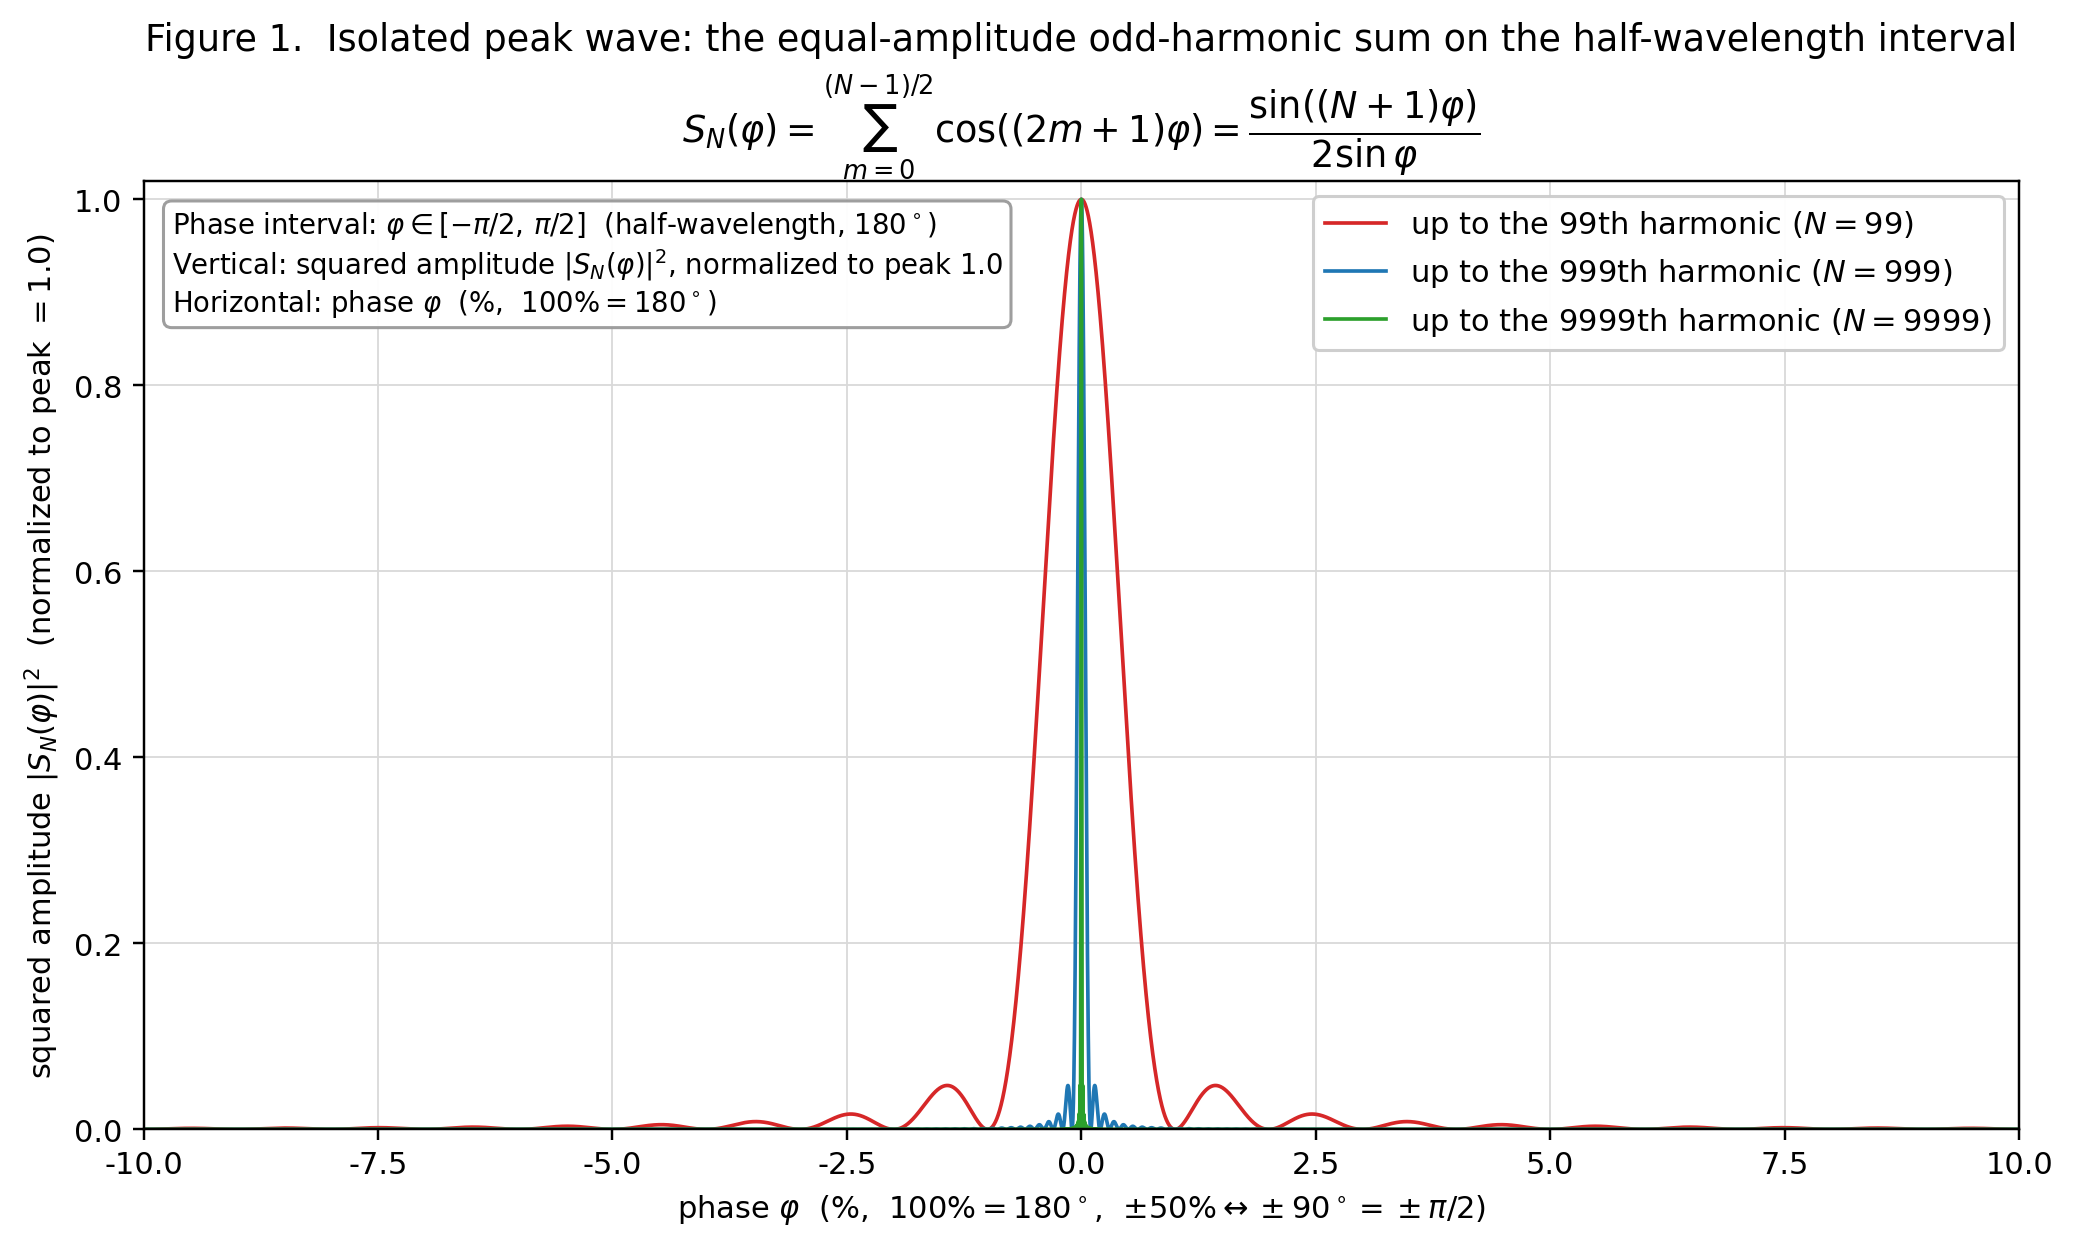
\includegraphics[keepaspectratio,alt={Figure 1}]{figures/fig01_odd_harmonic_localization.png}}
\caption{Figure 1}
\end{figure}

\textbf{Figure 1}: Isolated peak wave (the normalized squared amplitude
of the constant-amplitude odd-harmonic sum, \(N=99,\ 999,\ 9999\)).

\subsubsection{2.2 Cosine sum}\label{cosine-sum}

From the cosine-sum formula for the arithmetic progression \(a+md\)
(\(a=\varphi,\ d=2\varphi\)) {[}1{]},

\[
S_N(\varphi)=\sum_{m=0}^{(N-1)/2}\cos\!\big((2m+1)\varphi\big)
=\frac{\sin\!\big((N+1)\varphi\big)}{2\sin\varphi}
\tag{2.3}
\]

This Eq. (2.3) is an exact identity used repeatedly in what follows (at
\(\varphi=0\) the right-hand side is read as \(\lim_{\varphi\to0}\),
giving \(S_N(0)=(N+1)/2\) stated below).

\subsubsection{\texorpdfstring{2.3 The \(\sin u/u\) approximation near
the central main
peak}{2.3 The \textbackslash sin u/u approximation near the central main peak}}\label{the-sin-uu-approximation-near-the-central-main-peak}

Here we derive, step by step from Eq. (2.3), the approximate form used
in the later discussion of the localization width (§2.4). The goal is to
show that ``if we fix the magnified variable \(u=(N+1)\varphi\) and look
near the central main peak, then the shape of \(S_N\) normalized by its
peak value approaches the universal function \(\sin u/u\), independent
of \(N\).''

\textbf{Step 1 (magnified variable near the peak).} To observe only the
neighborhood of the central main peak (\(\varphi=0\)), introduce the
variable stretched to the peak width,

\[
u=(N+1)\varphi,\qquad\text{that is,}\quad \varphi=\frac{u}{N+1}
\tag{2.4}
\]

This is a magnifying lens that keeps the interior of the peak at a fixed
resolution however large \(N\) becomes; the range \(u=O(1)\) corresponds
to the neighborhood of the central main peak. Substituting into Eq.
(2.3), the numerator's argument \((N+1)\varphi\) becomes exactly \(u\),
so

\[
S_N(\varphi)=\frac{\sin\!\big((N+1)\varphi\big)}{2\sin\varphi}
=\frac{\sin u}{2\,\sin\!\big(u/(N+1)\big)}
\tag{2.5}
\]

This is still exact; no approximation has entered. The denominator
\(2\sin\varphi\) has not vanished but been rewritten as
\(2\sin\!\big(u/(N+1)\big)\).

\textbf{Step 2 (small-angle expansion of the denominator).} Keeping
\(u=O(1)\) (near the central main peak) and letting \(N\to\infty\), the
denominator's argument \(u/(N+1)\) becomes arbitrarily small. Applying
the small-angle expansion \(\sin\theta=\theta+O(\theta^3)\) with
\(\theta=u/(N+1)\),

\[
\sin\!\Big(\frac{u}{N+1}\Big)=\frac{u}{N+1}+O\!\Big(\frac{u^3}{(N+1)^3}\Big)
\tag{2.6}
\]

For \(u=O(1)\) (near the central main peak) the error is
\(O\!\big((N+1)^{-3}\big)\). Substituting into the denominator of Eq.
(2.5),

\[
S_N(\varphi)\approx\frac{\sin u}{2\,\dfrac{u}{N+1}}
=\frac{N+1}{2}\cdot\frac{\sin u}{u}
\tag{2.7}
\]

All \(N\)-dependence has collected into the prefactor
\(\tfrac{N+1}{2}\), and the \(u\)-dependent part has separated into the
universal form \(\sin u/u\), independent of \(N\).

\textbf{Step 3 (normalization by the peak value).} Since
\(\sin u/u\to1\) as \(u\to0\), the peak value is

\[
S_N(0)=\frac{N+1}{2}
\tag{2.8}
\]

(which also follows directly from each cosine in Eq. (2.1) being \(1\)
at \(\varphi=0\), with \((N+1)/2\) terms). To compare only the shape,
not the actual height of the wave, define the \textbf{normalized
amplitude} and \textbf{normalized squared amplitude}, divided by the
peak value, by

\[
\widehat{S}_N(\varphi):=\frac{S_N(\varphi)}{S_N(0)},
\qquad
\widehat{I}_N(\varphi):=\frac{I_N(\varphi)}{I_N(0)}=\widehat{S}_N(\varphi)^2
\]

(the vertical-axis normalization in Figures 1 and 2, and the
\(\widehat{I}_N\) used from Eq. (2.10) on, refer to this quantity).
Dividing Eq. (2.7) by Eq. (2.8), the prefactor \(\tfrac{N+1}{2}\)
cancels exactly, giving

\[
\widehat{S}_N(\varphi)\approx\frac{\sin u}{u},
\qquad
\widehat{I}_N(\varphi)=\widehat{S}_N(\varphi)^2\approx\Big(\frac{\sin u}{u}\Big)^2
\qquad(u=(N+1)\varphi)
\tag{2.9}
\]

This is the approximate form used from Eq. (2.10) on. The key points are
three: (i) the magnified variable \(u=(N+1)\varphi\) views the central
main peak at fixed resolution; (ii) under it the denominator
\(2\sin\varphi\) turns into \(2u/(N+1)\); and (iii) normalizing by the
peak value \(\tfrac{N+1}{2}\) makes the \(N\)-dependence drop out
completely. Moreover, that the pre-normalization localization width is
\(\varphi\sim u/(N+1)\), i.e.~shrinks as \(1/(N+1)\), can be read off
from Eq. (2.4).

Figure 2 shows (\(N=99,\ 999,\ 9999\)) together. The horizontal axis is
varied by factors of \(10\), \(\pm10\%,\ \pm1\%,\ \pm0.1\%\). The
vertical axis is shared across the three panels, with
\(|S_N(\varphi)|^2\) normalized to a maximum of \(1.0\). The figure is
to confirm visually that the width of the central main peak varies on
the \(1/(N+1)\) horizontal scale.

\begin{figure}
\centering
\pandocbounded{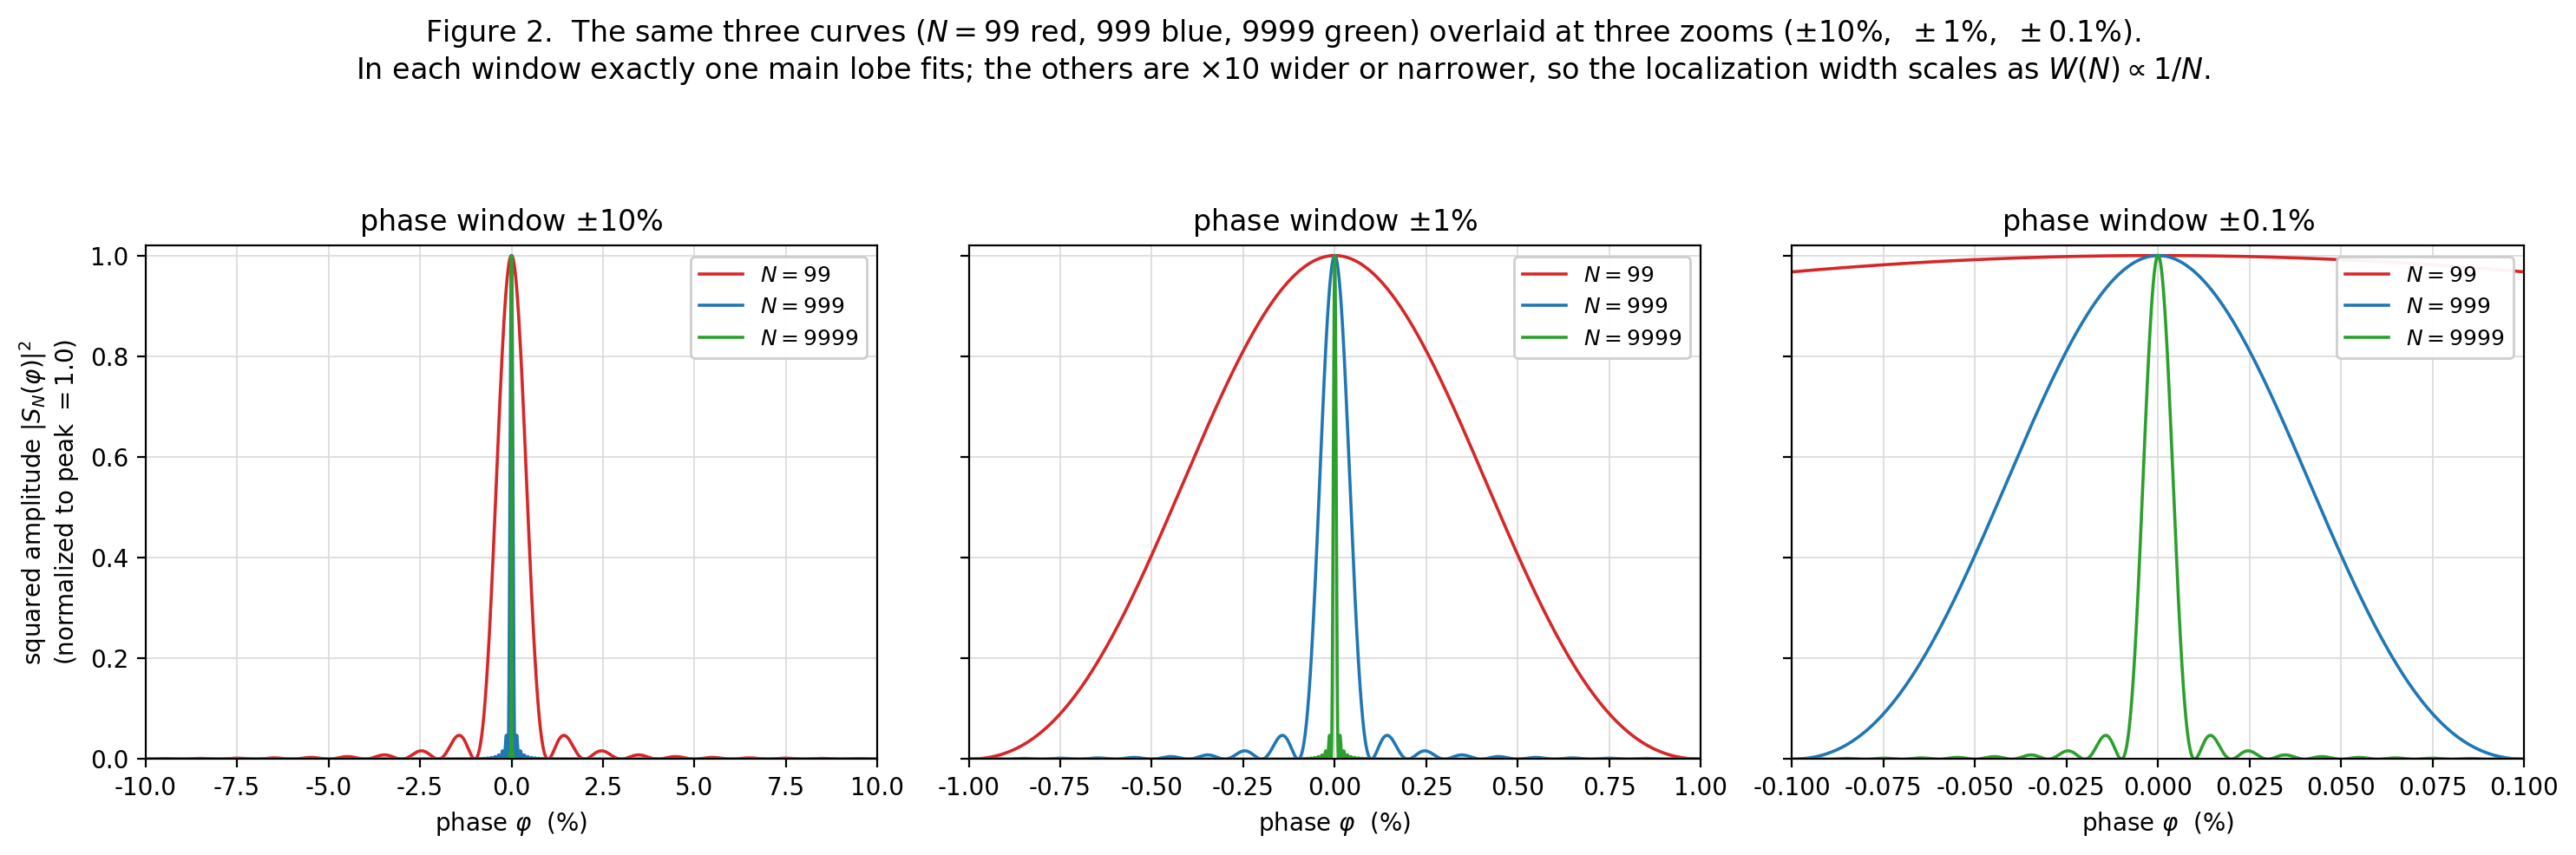
\includegraphics[keepaspectratio,alt={Figure 2}]{figures/fig02_odd_harmonic_scaling.png}}
\caption{Figure 2}
\end{figure}

\textbf{Figure 2}: \(1/(N+1)\) scaling of the localization width.

\subsubsection{\texorpdfstring{2.4 Required highest harmonic order
\(N_{\min}(\Delta_k,\,k)\) from a prescribed localization
width}{2.4 Required highest harmonic order N\_\{\textbackslash min\}(\textbackslash Delta\_k,\textbackslash,k) from a prescribed localization width}}\label{required-highest-harmonic-order-n_mindelta_kk-from-a-prescribed-localization-width}

We show how to solve ``how high must the highest odd-harmonic order
\(N\) be taken so that the normalized squared amplitude is held at or
below a tolerance level \(k\) outside a given phase.'' The key point is
that \(\widehat{I}_N\) has sidelobes (secondary maxima) outside the
central main lobe, so the sidelobes can exceed \(k\) far beyond the
position where the main lobe first drops through \(k\) (the main-peak
half-width of §2.3). Here \(\Delta_k\) is defined not as the main-lobe
half-width but as the \textbf{outermost edge, including sidelobes,
beyond which \(k\) is never exceeded again.}

Use the normalized phase \(x=\varphi/\pi\in[-\tfrac12,\tfrac12]\),
taking the full width \(\pi\) of the half-wavelength interval as \(1\).
For a tolerance level \(k\ (0<k<1)\), define the
\textbf{\(k\)-localization half-width} \(\Delta_k\) as the outermost
position at which the normalized squared amplitude exceeds \(k\),
i.e.~the largest solution of \(\widehat{I}_N(\pi x)=k\),

\[
\Delta_k=\max\{\,x\in(0,\tfrac12]:\ \widehat{I}_N(\pi x)=k\,\}
\qquad(\text{for}\ x>\Delta_k,\ \widehat{I}_N(\pi x)\le k)
\tag{2.10}
\]

This is ``the boundary phase, away from the center, beyond which
\(\widehat{I}_N\) no longer exceeds \(k\)'': not the first descent of
the main lobe, but the \textbf{last crossing}.

For large \(N\), by Eq. (2.9) of §2.3,
\[\widehat{I}_N(\varphi)\approx(\sin u/u)^2\qquad(u=(N+1)\varphi)\] so
\(\widehat{I}_N\) last exceeds \(k\) when \(u\) reaches the
\textbf{largest positive root} \(u_k^{\mathrm{out}}\) of

\[
\Big(\frac{\sin u_k^{\mathrm{out}}}{u_k^{\mathrm{out}}}\Big)^2=k
\tag{2.11}
\]

i.e.~at \(\varphi=u_k^{\mathrm{out}}/(N+1)\). Here
\(u_k^{\mathrm{out}}\) is the root on the descending flank of the
outermost sidelobe exceeding \(k\), a constant determined by the
tolerance level \(k\) alone (\(u_k^{\mathrm{out}}=8.423204\) for
\(k=0.01\) and \(30.151382\) for \(k=0.001\); by contrast the first
descent of the main lobe lies in \(u\in(0,\pi)\), only \(2.852342\) for
\(k=0.01\) and \(3.045147\) for \(k=0.001\)). Since \(g(u)=\sin u/u\) is
monotone only on \([0,\pi]\) and oscillates in the sidelobe region,
\(u_k^{\mathrm{out}}\) is not given by a single inverse function but is
the largest root, found numerically.

A closed-form upper bound follows from the sidelobe envelope. Since
\(|\sin((N+1)\varphi)|\le1\),

\[
\widehat{I}_N(\varphi)=\frac{\sin^2\!\big((N+1)\varphi\big)}{\big((N+1)\sin\varphi\big)^2}
\ \le\ \frac{1}{\big((N+1)\sin\varphi\big)^2},
\qquad
\Big(\frac{\sin u}{u}\Big)^2\le\frac{1}{u^2}
\tag{2.12}
\]

and this envelope decreases monotonically on \((0,\pi/2]\), reaching
\(k\) at \(u=1/\sqrt{k}\). Hence \(u_k^{\mathrm{out}}<1/\sqrt{k}\), and
using the envelope for \(\Delta_k\) is \textbf{conservative} (an
over-estimate that guarantees \(\widehat{I}_N\le k\)). For small \(k\)
the approximate closed form

\[
u_k^{\mathrm{out}}\approx\frac{1}{\sqrt{k}},\qquad\text{i.e.}\quad
\sin(\pi\Delta_k)\approx\frac{1}{(N+1)\sqrt{k}}
\tag{2.13}
\]

holds (the relative slack is \(\sim(\pi/2)\sqrt{k}\): about \(19\%\) at
\(k=0.01\), about \(4.9\%\) at \(k=0.001\), improving as \(k\)
decreases, and always on the safe side --- over-estimating \(N\)).

From the condition \(u_k^{\mathrm{out}}/(N+1)\le \pi\Delta_k\) that the
localization half-width be within \(\Delta_k\),

\[
N\ \ge\ \frac{u_k^{\mathrm{out}}}{\pi\,\Delta_k}-1
\tag{2.14}
\]

The form is the same as in the main-lobe case,
\(N=u^{\ast}/(\pi\Delta_k)-1\), but the essential change is that the
characteristic value passes from the main lobe's \(u_k\approx\pi\) to
the envelope / last-crossing value \(u_k^{\mathrm{out}}\) (about
\(8.42\) for \(k=0.01\), about \(30.2\) for \(k=0.001\)).

We distinguish two inversion methods. First, the method that uses the
largest root \(u_k^{\mathrm{out}}\) obtained by solving Eq. (2.11)
numerically is called here the \textbf{numerical-substitution method}.
It is defined by the single expression

\[
\begin{aligned}
N_{\mathrm{cont}}^{(\mathrm{num})}(\Delta_k,k)
&:=\frac{u_k^{\mathrm{out}}}{\pi\,\Delta_k}-1,
\qquad
\Big(\frac{\sin u_k^{\mathrm{out}}}{u_k^{\mathrm{out}}}\Big)^2=k,\quad u_k^{\mathrm{out}}=\text{largest positive root},\\
N_{\min}^{(\mathrm{num})}(\Delta_k,k)
&:=\min\Big\{\,N\in 2\mathbb{Z}_{\ge 0}+1:\ N\ge N_{\mathrm{cont}}^{(\mathrm{num})}(\Delta_k,k)\,\Big\}.
\end{aligned}
\tag{2.15}
\]

Here \(N_{\mathrm{cont}}^{(\mathrm{num})}\) is the continuous threshold
before imposing the odd-integer condition, and
\(N_{\min}^{(\mathrm{num})}\) is the smallest odd integer at least as
large. This inversion formula uses the numerical solution (largest root)
of Eq. (2.11) directly, without replacing \(u_k^{\mathrm{out}}\) by
elementary functions.

Second, substituting the envelope approximation (2.13) to eliminate
\(u_k^{\mathrm{out}}\) yields the \textbf{approximate closed form}

\[
N_{\mathrm{cont}}^{(\mathrm{app})}(\Delta_k,k)
:=\frac{1}{\sqrt{k}\,\sin(\pi\Delta_k)}-1
\ \approx\ \frac{1}{\pi\sqrt{k}\,\Delta_k}-1
\tag{2.16}
\]

Eq. (2.16) is a \textbf{conservative over-estimate} stemming from the
envelope upper bound (about \(+19\%\) at \(k=0.01\), about \(+4.9\%\) at
\(k=0.001\), improving for small \(k\)), useful as a simple closed form
when one wants to rigorously guarantee \(\widehat{I}_N\le k\). For the
exact required order, use the numerical-substitution method (2.15).

Adding \(N=99999,\ 999999\) to the \(N=99,\ 999,\ 9999\) used in Figures
1 and 2, and taking the localization half-width \(\Delta_{0.01}\) at
\(k=0.01\) (the last crossing, evaluated from the exact
\(\widehat{I}_N\)) as input, the numerical-substitution method (2.15)
and the approximate closed form (2.16) compare as follows:

{\def\LTcaptype{none} % do not increment counter
\begin{longtable}[]{@{}
  >{\raggedleft\arraybackslash}p{(\linewidth - 8\tabcolsep) * \real{0.2000}}
  >{\raggedleft\arraybackslash}p{(\linewidth - 8\tabcolsep) * \real{0.2000}}
  >{\raggedleft\arraybackslash}p{(\linewidth - 8\tabcolsep) * \real{0.2000}}
  >{\raggedleft\arraybackslash}p{(\linewidth - 8\tabcolsep) * \real{0.2000}}
  >{\raggedleft\arraybackslash}p{(\linewidth - 8\tabcolsep) * \real{0.2000}}@{}}
\toprule\noalign{}
\begin{minipage}[b]{\linewidth}\raggedleft
Original highest odd-harmonic order \(N\)
\end{minipage} & \begin{minipage}[b]{\linewidth}\raggedleft
\(\Delta_{0.01}\) (last crossing, exact evaluation, percent)
\end{minipage} & \begin{minipage}[b]{\linewidth}\raggedleft
\(N_{\mathrm{cont}}^{(\mathrm{num})}\) (Eq. (2.15))
\end{minipage} & \begin{minipage}[b]{\linewidth}\raggedleft
\(N_{\min}^{(\mathrm{num})}\) (Eq. (2.15))
\end{minipage} & \begin{minipage}[b]{\linewidth}\raggedleft
\(N_{\mathrm{cont}}^{(\mathrm{app})}\) (Eq. (2.16))
\end{minipage} \\
\midrule\noalign{}
\endhead
\bottomrule\noalign{}
\endlastfoot
\(99\) & \(2.6816849\%\) & \(98.981512\) & \(99\) & \(117.838252\) \\
\(999\) & \(0.2681194\%\) & \(998.998149\) & \(999\) &
\(1186.208552\) \\
\(9999\) & \(0.0268119\%\) & \(9998.999815\) & \(9999\) &
\(11870.968289\) \\
\(99999\) & \(0.0026812\%\) & \(99998.999981\) & \(99999\) &
\(118718.671164\) \\
\(999999\) & \(0.0002681\%\) & \(999998.999998\) & \(999999\) &
\(1187195.710468\) \\
\end{longtable}
}

The numerical-substitution method (2.15) recovers the original \(N\)
almost exactly (the slight undershoot at \(N=99\) is because the last
crossing lies outside the main lobe, where \(\varphi\) is larger, so the
small-angle error of the \(\sin u/u\) approximation is larger than for
the main-lobe half-width; it disappears as \(N\) grows). The approximate
closed form (2.16) is consistently about \(1.19\times\) (\(+19\%\))
larger, i.e.~on the safe side.

\begin{center}\rule{0.5\linewidth}{0.5pt}\end{center}

\subsection{3. Conclusion}\label{conclusion}

For the constant-amplitude odd-harmonic sum on the half-wavelength phase
interval \(\varphi\in[-\pi/2,\pi/2]\),

\[
S_N(\varphi)=\sum_{m=0}^{(N-1)/2}\cos\!\big((2m+1)\varphi\big)
\]

we obtained the following results.

\textbf{(1) Formation of the isolated peak wave}

\begin{itemize}
\tightlist
\item
  \(S_N\) is an ``isolated peak wave'' with a main peak at the center,
  \(S_N(0)=(N+1)/2\), and zeros at both ends.
\end{itemize}

\textbf{(2) Period and fundamental domain of the squared amplitude}

\begin{itemize}
\tightlist
\item
  The squared amplitude \(I_N=|S_N|^2\) has period \(\pi\), and the
  half-wavelength interval \([-\pi/2,\pi/2]\) is its fundamental domain.
\end{itemize}

\textbf{(3) Cosine sum}

\begin{itemize}
\tightlist
\item
  By the cosine-sum formula for an arithmetic progression (Eq. (2.3)),
  \(S_N(\varphi)=\sin\!\big((N+1)\varphi\big)/(2\sin\varphi)\).
\end{itemize}

\textbf{(4) Normalized form near the central main peak}

\begin{itemize}
\tightlist
\item
  With the magnified variable \(u=(N+1)\varphi\), for large \(N\) the
  normalized amplitude is \(\widehat{S}_N(\varphi)\approx \sin u/u\) and
  the normalized squared amplitude is
  \(\widehat{I}_N(\varphi)\approx(\sin u/u)^2\) (Eq. (2.9)). At the same
  time, the horizontal width of the central main peak shrinks on the
  \(1/(N+1)\) scale.
\end{itemize}

\textbf{(5) Inverse formula for the required harmonic order}

\begin{itemize}
\tightlist
\item
  Solve for \(N\) from a target localization half-width \(\Delta_k\)
  (the \textbf{last crossing} beyond which \(k\) is never exceeded again
  --- the outer edge where the sidelobe envelope finally falls to \(k\),
  lying outside the main-lobe half-width) and tolerance level \(k\). The
  characteristic value is the last crossing \(u_k^{\mathrm{out}}\) (the
  largest root of \((\sin u/u)^2=k\)), with
  \(N=u_k^{\mathrm{out}}/(\pi\Delta_k)-1\) (numerical-substitution
  method, Eq. (2.15)). A conservative approximate closed form
  \(N\approx1/(\pi\sqrt{k}\,\Delta_k)-1\) from the envelope upper bound
  \(u_k^{\mathrm{out}}\lesssim1/\sqrt{k}\) (Eq. (2.16)) is also given.
\end{itemize}

All of these are elementary properties of Fourier sums, and no physical
interpretation is given.

\begin{center}\rule{0.5\linewidth}{0.5pt}\end{center}

\subsection{References}\label{references}

{[}1{]} Teiji Takagi, \emph{Kaiseki Gairon} (Introduction to Analysis),
3rd revised ed., Iwanami Shoten, 1961 (the chapter on Fourier series:
trigonometric series, the closed form of cosine sums, the Dirichlet
kernel, and the expansion of the square wave).

\begin{center}\rule{0.5\linewidth}{0.5pt}\end{center}

\subsection{Appendix A: Scale estimates (numerical example; not a
physical
claim)}\label{appendix-a-scale-estimates-numerical-example-not-a-physical-claim}

The following is merely a \textbf{numerical example} to show the reach
of the numerical-substitution method \textbf{Eq. (2.15)}. It does not
claim any particular physical system or physical correspondence.

Let the full width of the half-wavelength interval correspond to some
large length \(L\) (regarded as a half-wavelength), and consider
squeezing the central isolated peak wave to a half-width of order the
Bohr radius \(a_0\approx5.29\times10^{-11}\,\mathrm{m}\), used here for
convenience as an example of an arbitrary small length scale (the Bohr
radius is only one example of a concrete small scale and does not denote
any particular physical object). Then, since the half-wavelength
interval (full width \(\pi\)) corresponds to the physical length \(L\),
the normalized half-width is \(\Delta_k=a_0/L\).

For each row, substitute \(k=0.01\) and \(\Delta_k=a_0/L\) into Eq.
(2.15) to compute \(N_{\mathrm{cont}}^{(\mathrm{num})}\). To obtain the
required highest odd-harmonic order as an integer, choose, per (2.15),
the smallest odd integer \(N_{\min}^{(\mathrm{num})}\) at least equal to
\(N_{\mathrm{cont}}^{(\mathrm{num})}\).

Numerical example (target half-width \(=a_0\), \(k=1\%\), computed by
Eq. (2.15)):

{\def\LTcaptype{none} % do not increment counter
\begin{longtable}[]{@{}
  >{\raggedright\arraybackslash}p{(\linewidth - 8\tabcolsep) * \real{0.1579}}
  >{\raggedleft\arraybackslash}p{(\linewidth - 8\tabcolsep) * \real{0.2105}}
  >{\raggedleft\arraybackslash}p{(\linewidth - 8\tabcolsep) * \real{0.2105}}
  >{\raggedleft\arraybackslash}p{(\linewidth - 8\tabcolsep) * \real{0.2105}}
  >{\raggedleft\arraybackslash}p{(\linewidth - 8\tabcolsep) * \real{0.2105}}@{}}
\toprule\noalign{}
\begin{minipage}[b]{\linewidth}\raggedright
Half-wavelength \(L\)
\end{minipage} & \begin{minipage}[b]{\linewidth}\raggedleft
\(L\) {[}m{]}
\end{minipage} & \begin{minipage}[b]{\linewidth}\raggedleft
\(L/a_0\)
\end{minipage} & \begin{minipage}[b]{\linewidth}\raggedleft
\(\Delta_k=a_0/L\)
\end{minipage} & \begin{minipage}[b]{\linewidth}\raggedleft
\(N_{\mathrm{cont}}^{(\mathrm{num})}\)
\end{minipage} \\
\midrule\noalign{}
\endhead
\bottomrule\noalign{}
\endlastfoot
\(1\) light-year & \(9.46\times10^{15}\) & \(1.79\times10^{26}\) &
\(5.59\times10^{-27}\) & \(\sim 4.8\times10^{26}\) \\
Radius of the observable universe & \(4.4\times10^{26}\) &
\(8.3\times10^{36}\) & \(1.2\times10^{-37}\) &
\(\sim 2.2\times10^{37}\) \\
\(2\times10^{11}\) light-years & \(1.89\times10^{27}\) &
\(3.58\times10^{37}\) & \(2.79\times10^{-38}\) &
\(\sim 9.6\times10^{37}\) \\
\end{longtable}
}

For example, at \(L=2\times10^{11}\) light-years (merely an image of the
size of the universe including unobservable regions), target half-width
\(=\) Bohr radius, and \(k=1\%\), the normalized half-width is
\(\Delta_k=a_0/L\approx2.79\times10^{-38}\), and, using the \(k=0.01\)
last crossing \(u_k^{\mathrm{out}}=8.423204\), the continuous value of
Eq. (2.15) is
\(N_{\mathrm{cont}}^{(\mathrm{num})}\approx9.6\times10^{37}\). The
required order \(N\) is proportional to the half-wavelength \(L\) and
inversely proportional to the target half-width.

To repeat, this appendix is an arithmetic application of the
numerical-substitution method (Eq. (2.15)) to given scale ratios, and
does not claim physical reality or any physical process.

\begin{center}\rule{0.5\linewidth}{0.5pt}\end{center}

\subsection{Appendix B: Reproducing the
figures}\label{appendix-b-reproducing-the-figures}

Figure 1 is generated by \texttt{figures/make\_odd\_harmonic\_figure.py}
and Figure 2 by \texttt{figures/make\_odd\_harmonic\_scaling\_figure.py}
(outputs: \texttt{figures/fig01\_odd\_harmonic\_localization.png} /
\texttt{.svg} and \texttt{figures/fig02\_odd\_harmonic\_scaling.png} /
\texttt{.svg}). Both plot, on the half-wavelength interval
\(\varphi\in[-\pi/2,\pi/2]\) (horizontal axis \(100\%=180^\circ\),
\(\pm50\%\leftrightarrow\pm90^\circ\)), the amplitude \(S_N\) evaluated,
squared, and normalized to a maximum of \(1.0\). Figure 2 has three
panels with the horizontal axis taken as \(\pm10\%,\ \pm1\%,\ \pm0.1\%\)
(by factors of \(10\)) for \(N=99,\ 999,\ 9999\). Each script first
verifies that, for each \(N\), the direct sum of Eq. (2.1) and the
closed form of Eq. (2.3) agree to machine precision (maximum absolute
difference \(\lesssim 10^{-9}\)) before plotting.

\end{document}
